\documentclass{article}
\usepackage[utf8]{inputenc}
\usepackage{graphicx}
\graphicspath{{./images/}}

\title{PS6_Castiglione}
\author{joe.castiglione.jr }
\date{March 2020}

\begin{document}

\maketitle

\section{Steps to Clean Data}
I chose to use the data that I scraped from the last problem set. This was a table from USA Today that included the strength coach salaries for Division 1 football programs. First off to clean the data I removed the dollar signs from the column knowing that R would not recognize them.Then proceeded to make the edited columns the new ones.  After that I went and removed the empty values and replaced them with NA. Finally there was a random row with unnecessary information I took out. 

\section{Visualisations Explanation}
Histogram - I chose to use an histogram because while it is not always the most intuitive, it is always easy to make some rough hypothesis about data. I wanted to see the overall trend of salaries and see if it was normally distributed. Box Plot- This was to get an overall feel to find out the range of the salaries based on conference. Scatter plot - For this visualization I wanted to go one step further and seeing the specific salaries of each conference. 

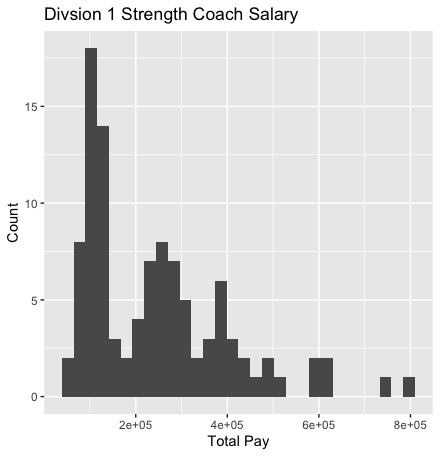
\includegraphics[]{vis 1.png}
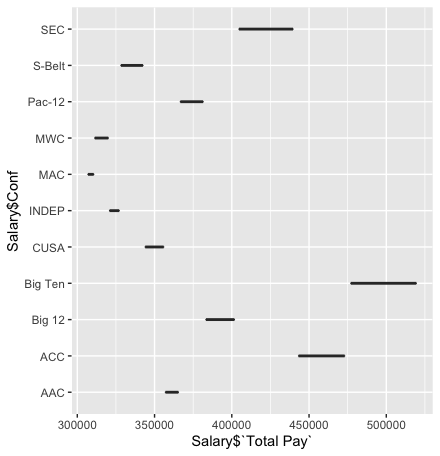
\includegraphics[]{Vis 2.png}
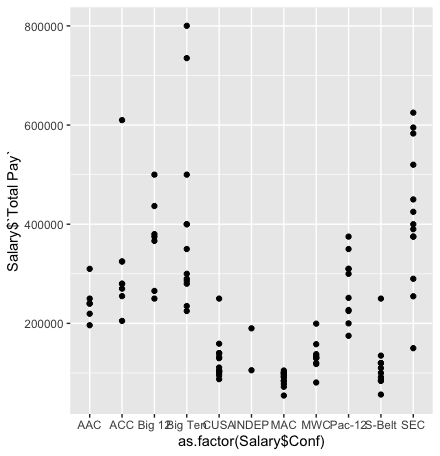
\includegraphics[]{Vis 3.png}

\end{document}
